\documentclass[12pt]{article}
\usepackage[margin=1in]{geometry}
\usepackage{tikz}
\usetikzlibrary{shapes.geometric, arrows.meta, positioning}

\tikzstyle{topic}=[rectangle, rounded corners, draw=blue!70!black, fill=blue!5, thick, text width=4cm, align=center, minimum height=1cm]
\tikzstyle{arrow}=[->, thick, >=Stealth]

\begin{document}
{\large \textbf{Discrete Structures \quad Chapter 4.6 — Cryptography Summary Diagram}}

\hrule
\vspace{1em}

\begin{center}
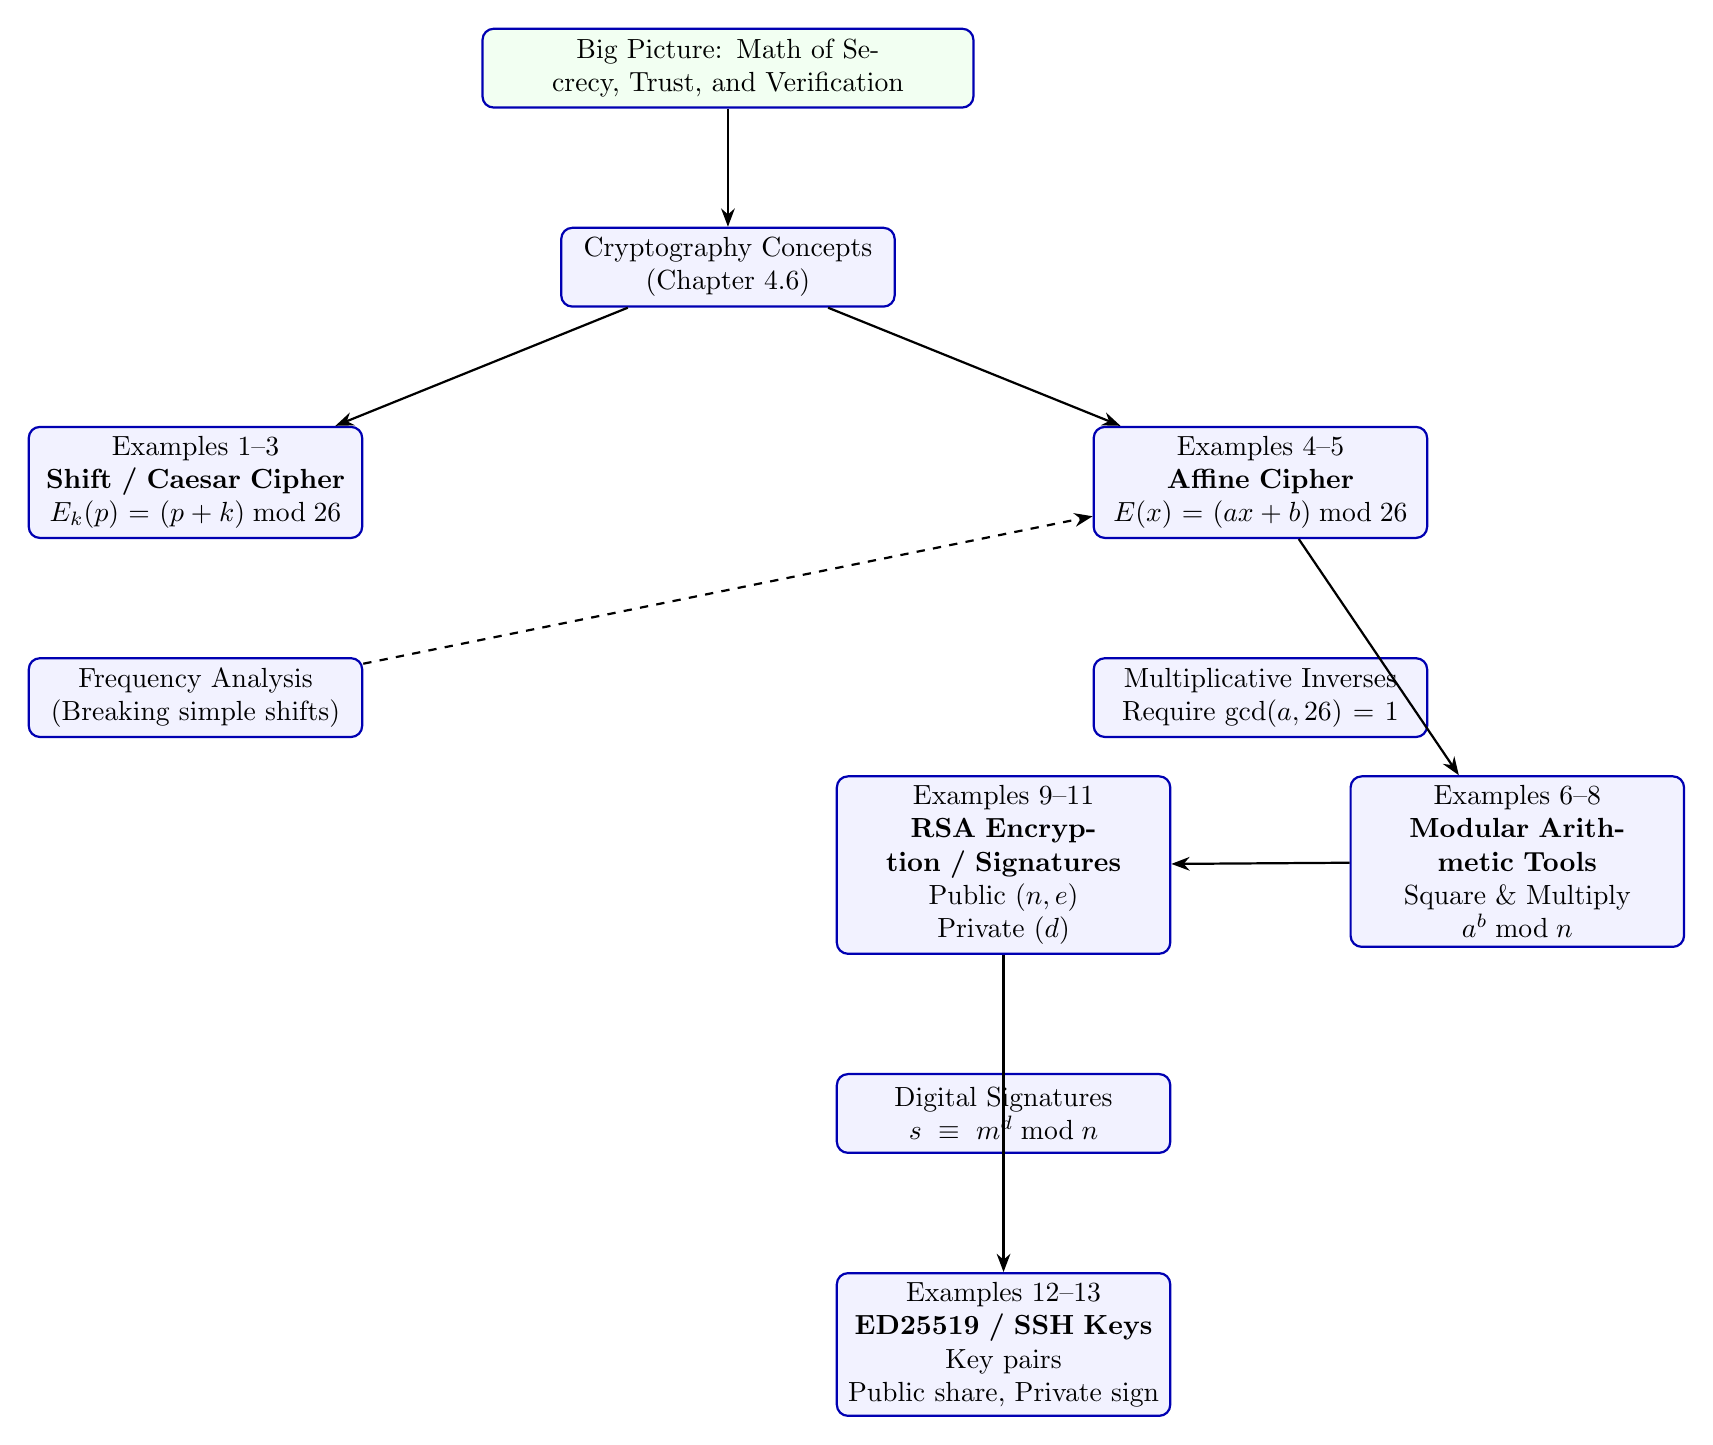
\begin{tikzpicture}[node distance=1.5cm and 2.5cm]

% Core
\node[topic] (core) {Cryptography Concepts \\ (Chapter 4.6)};

% Caesar / Shift
\node[topic, below left=of core] (caesar) {Examples 1–3 \\ \textbf{Shift / Caesar Cipher} \\ $E_k(p)=(p+k)\bmod26$};
\node[topic, below=of caesar] (freq) {Frequency Analysis \\ (Breaking simple shifts)};

% Affine
\node[topic, below right=of core] (affine) {Examples 4–5 \\ \textbf{Affine Cipher} \\ $E(x)=(ax+b)\bmod26$};
\node[topic, below=of affine] (inv) {Multiplicative Inverses \\ Require $\gcd(a,26)=1$};

% Modular Arithmetic
\node[topic, below right=3cm and -1cm of affine] (mod) {Examples 6–8 \\ \textbf{Modular Arithmetic Tools} \\ Square \& Multiply \\ $a^b\bmod n$};

% RSA
\node[topic, below left=3cm and -1cm of affine] (rsa) {Examples 9–11 \\ \textbf{RSA Encryption / Signatures} \\ Public $(n,e)$ \quad Private $(d)$};
\node[topic, below=of rsa] (sig) {Digital Signatures \\ $s \equiv m^d \bmod n$};

% SSH Keys
\node[topic, below=of sig] (ssh) {Examples 12–13 \\ \textbf{ED25519 / SSH Keys} \\ Key pairs \\ Public share, Private sign};

% Flow arrows
\draw[arrow] (core) -- (caesar);
\draw[arrow] (core) -- (affine);
\draw[arrow] (affine) -- (mod);
\draw[arrow] (mod) -- (rsa);
\draw[arrow] (rsa) -- (ssh);
\draw[arrow, dashed] (freq) -- (affine);

% Context note
\node[topic, above=of core, fill=green!5, text width=6cm] (bigpic) {Big Picture: Math of Secrecy, Trust, and Verification};

\draw[arrow] (bigpic) -- (core);

\end{tikzpicture}
\end{center}

\vspace{1em}
\hrule
\vspace{0.6em}

\textbf{Reading tip:} Follow the arrows downward to see how we evolve from simple shifts to full modern public–private key cryptography.  
Each stage adds new mathematical tools — from modular addition, to inverses, to exponentiation, to prime-based encryption, and finally to elliptic curves.

\end{document}

